\section{Memmory flatenig}

A common problem in multidimensional data situations is memmory layout representation. Internally computers always represnt memorry in a linear fashion, the idea of mutidimensional array is just sugar syntax added by high level programming lenguajes.

Given said that, sometimes such allocations can become dificult to use or declare by themselves. Especially in C++. Lets see an example:

{\centering
\begin{minipage}{\linewidth}
  \begin{listing}[H]
  \inputminted[
  xleftmargin=1.5cm,  %without this option line number goes wrong
  %frame=lines,
  framesep=0.5cm,
  baselinestretch=1.2,
  %fontsize=\footnotesize,
  linenos,
  firstline=15, %If you omit this two fields, the whole file is pulled
  lastline=21
  ]{cpp}{src/ArrayDimensions.cpp}
  \caption{One dimensioal array (by means of \mintinline{cpp}{std::vector} class) used}
  \label{lst:1Dexample}
  \end{listing}
\end{minipage}
\par
}
\vspace{0.5cm}
So far, everything looks good, sintax is clear, braket operator is helping us. 
Conceptually, we have a series of variables with the same type that live in a contiguos space in memmory. See figure~\ref{fig:1D}.

\begin{figure}[htp]
  \centering
  \begin{subfigure}[b]{0.35\textwidth}
    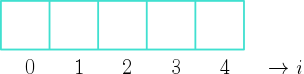
\includegraphics[width=\textwidth]{img/array1D}
    \caption{Logical memmory layout representation.}
  \label{fig:1a}
  \end{subfigure}
  \hspace*{4cm}
  \begin{subfigure}[b]{0.25\textwidth}
    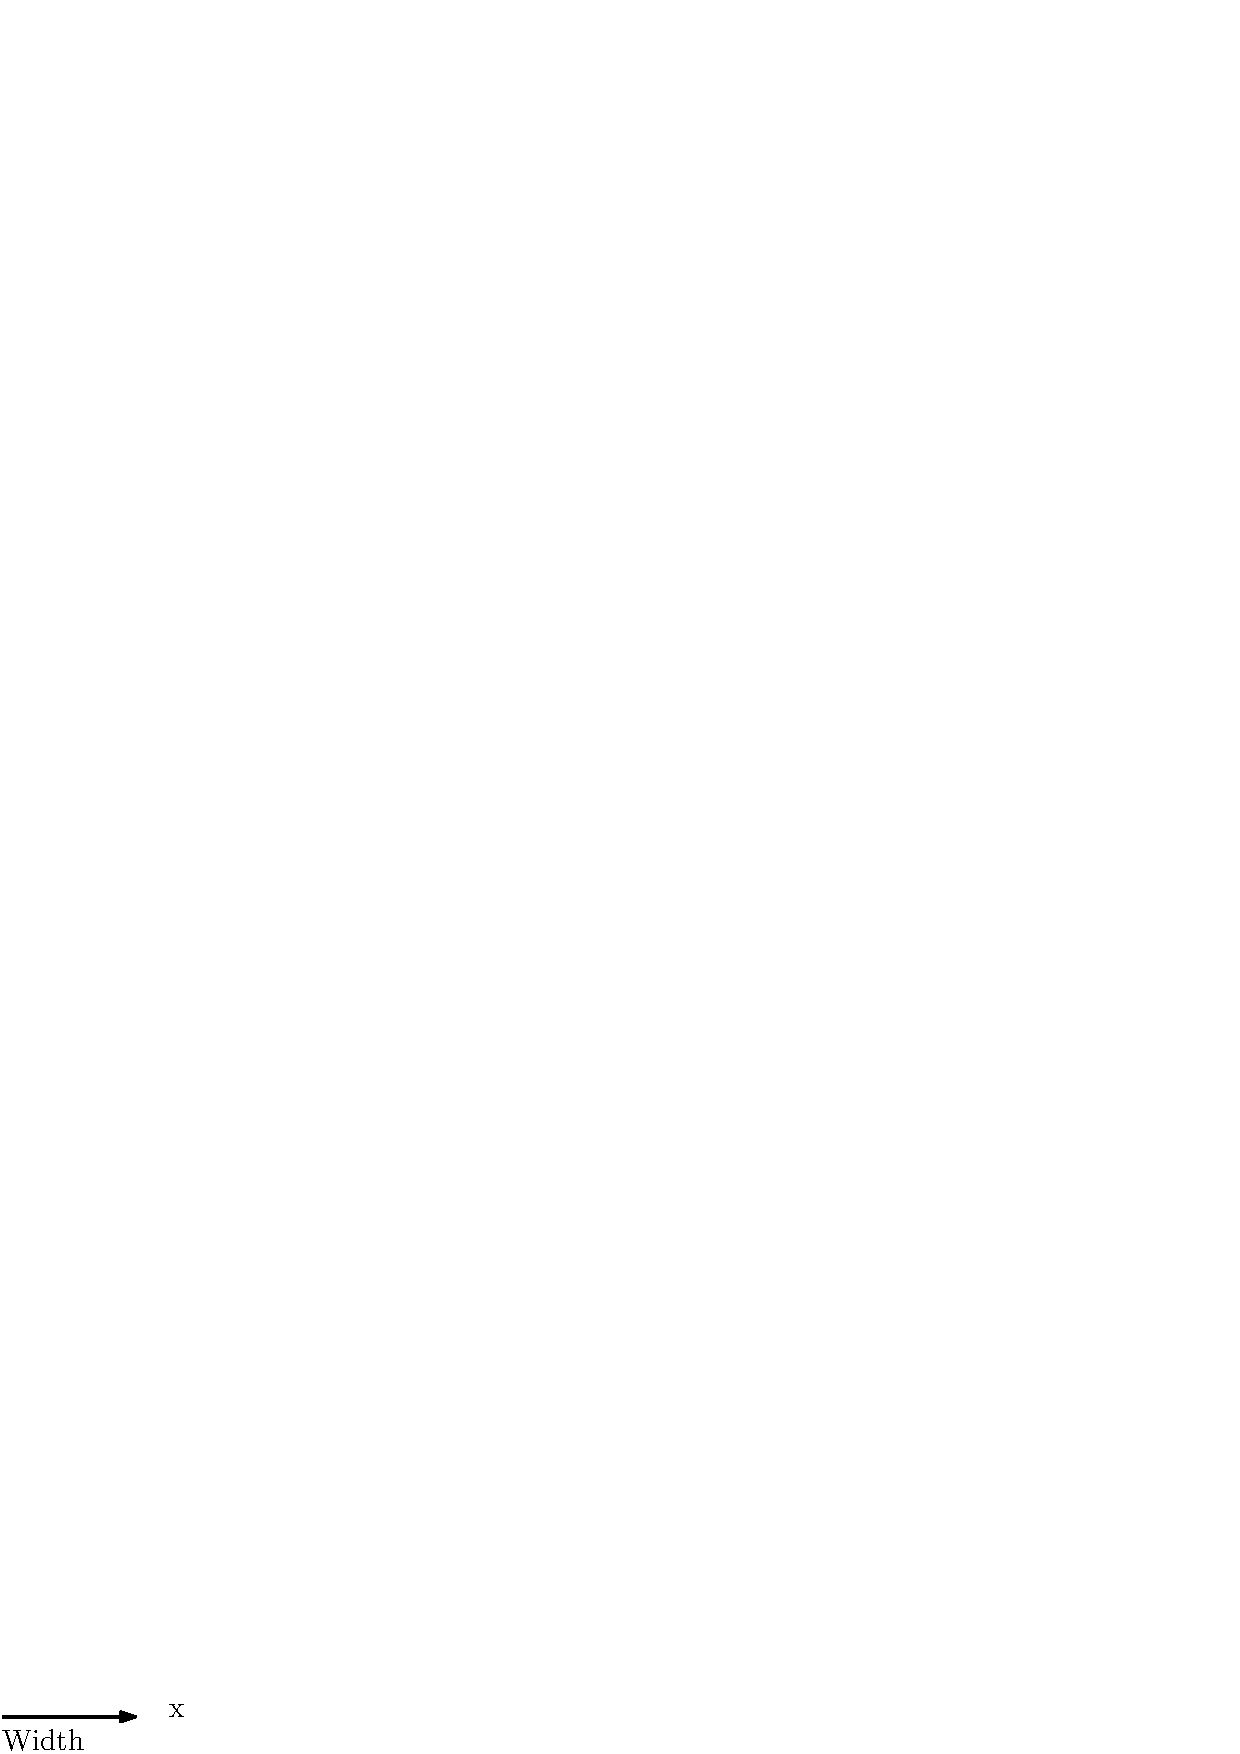
\includegraphics[width=\textwidth]{img/arrow1D}
    \caption{Dimensions represented.}
    \label{fig:1b}
  \end{subfigure}
  \caption{One dimensional array representation.}
  \label{fig:1D}
\end{figure}

The problem will start to become aparent as data start to include more dimensions. 
In a bidimensional array we have data that has two dimensions.
One can think about it like it's on a table, the situation is the one depicted in Figure~\ref{fig:2a}. 
Now, remember this is just an abstraction (provided by our programming language; C++ in this case), since memmory is always linear in the computer.

\begin{figure}[htp]
  \centering
  \begin{subfigure}[b]{0.35\textwidth}
    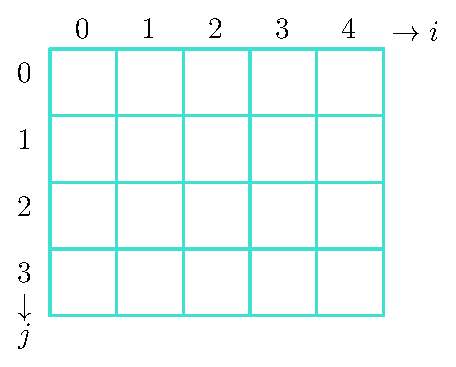
\includegraphics[width=\textwidth]{img/array2D}
    \caption{Logical memmory layout representation.}
  \label{fig:2a}
  \end{subfigure}
  \hspace*{4cm}
  \begin{subfigure}[b]{0.25\textwidth}
    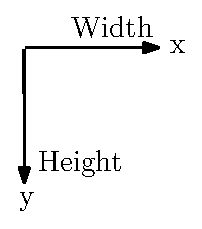
\includegraphics[width=\textwidth]{img/arrow2D}
    \caption{Dimensions represented.}
    \label{fig:2b}
  \end{subfigure}
  \caption{Two dimensional array representation.}
  \label{fig:2D}
\end{figure}

Usually, the C++ way of modeling this is creating an array, such that each element of it is also an array. See the code in Listing~\ref{lst:2dexample}

{\centering
\begin{minipage}{\linewidth}
  \begin{listing}[H]
  \inputminted[
  xleftmargin=1.5cm,  %without this option line number goes wrong
  %frame=lines,
  framesep=0.5cm,
  baselinestretch=1.2,
  %fontsize=\footnotesize,
  linenos,
  firstline=23, %If you omit this two fields, the whole file is pulled
  lastline=38
  ]{cpp}{src/ArrayDimensions.cpp}
  \caption{Two dimensioal array example}
  \label{lst:2dexample}
  \end{listing}
\end{minipage}
\par
}
\vspace{0.5cm}
Now, there is two main points to highlight in the sample:
\begin{enumerate}
 \item Type of the array has change. Now is \emph{a vector of int vectors}. This led us to have a longer initialization for it too. Imagine that you create functions to receive or return such arrays (Sintax to declare the parameters become difficult)
 \item We still have the huge advantage of a very elegant sintax to use the array: \mintinline{cpp}{b[j][i]} give us the element on column $i$ of row $j$ (We are zero based).
\end{enumerate}
Here is when the technique called memmory flattening becomes useful
\begin{figure}[htp]
  \centering
  \begin{subfigure}[b]{0.35\textwidth}
    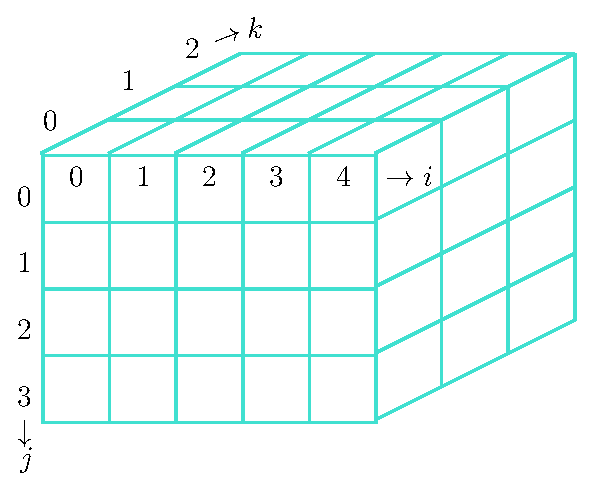
\includegraphics[width=\textwidth]{img/array3D}
    \caption{Logical memmory layout representation.}
  \label{fig:3a}
  \end{subfigure}
  \hspace*{4cm}
  \begin{subfigure}[b]{0.2\textwidth}
    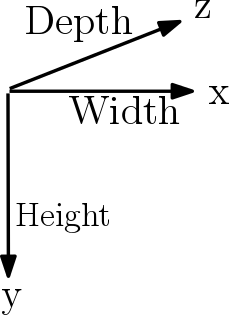
\includegraphics[width=\textwidth]{img/arrow3D}
    \caption{Dimensions represented.}
    \label{fig:3b}
  \end{subfigure}
  \caption{Three dimensional array representation.}
  \label{fig:3D}
\end{figure}

\section{Bit Shifting}
\section{Analytic Geometry}
\section{Graphics Pipeline}
